\chapter{Arquitetura para compartilhamento de informações do ativo}
\label{cha:arquitetura}
	
	A elaboração de uma arquitetura comum para o compartilhamento de informações do ativo é essencial para que haja consistência e interoperabilidade entre os membros da Cadeia de Suprimentos (CS) adotando este sistema.
	
	Este capítulo tem o objetivo de apresentar detalhes da arquitetura proposta baseada em \textit{Web Services} (WS) nos modelos de uma arquitetura orientada a serviços (SOA) compatível com Componentes I4.0 para o compartilhamento de informações do ativo ao longo da CS. A fim de simplificação do texto, os \textit{Web Services} serão mencionados apenas como ``serviços''.
	
	Neste capítulo é apresentado também o mapeamento dos componentes desta arquitetura dentro do eixo camadas do RAMI4.0.
	
\section{Componentes e operações de serviços dos AASs}

	Os serviços no escopo desta arquitetura são representações das funcionalidades dos Componentes I4.0 e são fornecidos e consumidos entre \textit{Asset Administration Shells} (AASs).
	
	A lógica de fornecimento e consumo de serviços proposta para a I4.0 segue os moldes de um \textit{Web Service} explicado na \autoref{sec:webservices}, apresentando os componentes e operações (vide \autoref{fig:webservice-componentes}) adaptados ao AAS.
	
	Esta arquitetura envolve três componentes (atores) básicos: O AAS cliente, o AAS servidor e o AAS repositório; e três operações: publicação, busca e interação.

	Os serviços disponibilizados remotamente pelo AAS servidor escuta e responde solicitações de clientes por meio de uma determinada rede e porta. Os AAS clientes, por sua vez, consomem o serviço disponibilizado pelo servidor por meio de solicitações.
	
	Nesta seção são apresentados detalhes sobre os componentes e operações necessárias para o fornecimento serviços no mundo conectado da I4.0.
	
\subsection{Componentes}

	Os componentes da arquitetura e suas inter-relações são apresentados na \autoref{fig:aas-ws}.
	
	\begin{figure}[htb]
		\centering
		\caption{Componentes e operações do WS.}
		\label{fig:aas-ws}
		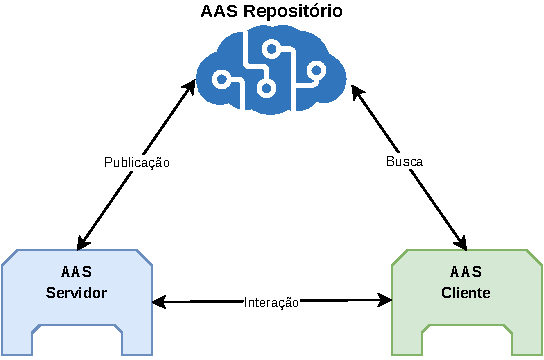
\includegraphics[width=0.7\textwidth]{aas-ws}
		\fonte{O autor.}
	\end{figure}

	De maneira sucinta, os componentes são descritos da seguinte forma: ``O AAS Servidor'' é a parte que possui um serviço a oferecer para os demais AASs no mundo conectado, o ``AAS Cliente'' é a parte que necessita de um serviço e que age ativamente para receber este serviço e o ``AAS Repositório'' é a parte que armazena informações sobre descrições de diversos serviços.
	
	A \autoref{tab:componentes-ws} lista os componentes da arquitetura para a I4.0 e suas respectivas descrições detalhadas.
	
	\begin{table}[htb]
		\centering
		\caption{Componentes da arquitetura para a I4.0.}
		\label{tab:componentes-ws}
		\begin{tabular}{p{3cm}p{12cm}}
			\hline
			\textbf{Componente}
			& \textbf{Descrição} \\ 
			
			\hline
			AAS Servidor
			& O AAS Servidor é a conexão direta com o ativo. Este AAS extrai as informações sobre seu ativo para sua própria MDP para que assim possam ser disponibilizadas na rede. Cada submodelo do AAS representa um conjunto de informações e serviços semelhantes agrupados. \\
			
			\hline
			AAS Cliente
			& O AAS Cliente é a parte que irá consumir as informações disponibilizadas pelo AAS Servidor. O cliente representa cada uma das partes envolvidas na cadeia de suprimentos. Pode representar uma instituição, uma pessoa física ou até mesmo uma outra máquina/produto. \\
			
			\hline
			AAS Repositório
			& O repositório é o componente que recebe, armazena e disponibiliza informações de descrição sobre todos os serviços disponíveis no mundo conectado. O AAS recebe operações de ``publicação'' por parte do AAS Servidor e operações de ``busca'' por parte do AAS Cliente. O Repositório não atua como canal de comunicação entre AAS Cliente e Servidor, mas apenas fornece informações necessárias para que ambos os AAS possam se comunicar diretamente por meio da operação de ``interação''. \\
			
			\hline
		\end{tabular}
		\fonte{O autor.}
	\end{table}
	
	Neste modelo, a descrição dos serviços disponíveis nos submodelos de cada AAS é armazenada em um repositório comum, onde todos os AASs disponíveis no mundo conectado na I4.0 poderiam se tornar visíveis. A função do repositório é armazenar uma descrição dos serviços disponíveis e não o serviço em si. O serviço é fornecido pelo próprio AAS Servidor que o disponibilizou, servindo o repositório apenas como um elemento para a descoberta de serviços.

	Cada AAS pode atuar tanto como um fornecedor de serviços (servidor), quanto como um solicitante de serviços (cliente), ou como ambos. Sempre usando o repositório como meio para a publicação ou busca dos serviços.

\subsection{Operações}

	As operações de serviços de AASs e suas inter-relações com os componentes são mostradas por meio dos arcos na \autoref{fig:aas-ws} e suas descrições detalhadas são apresentadas na \autoref{tab:operacoes-ws}
	
	\begin{table}[htb]
		\centering
		\caption{Operações do WS para a I4.0.}
		\label{tab:operacoes-ws}
		\begin{tabular}{p{3cm}p{12cm}}
			\hline
			\textbf{Operação}
			& \textbf{Descrição} \\ 
			
			\hline
			Publicação
			& Ação tomada pelo AAS Servidor sempre que este componente queira anunciar um serviço para que possa ser descoberto. Nesta operação, o AAS Servidor envia uma lista de seus serviços ofertados e a descrição de cada um desses serviços. Esta lista é recebida e armazenada pelo AAS Repositório, que a disponibiliza para acesso público. \\
			
			\hline
			Busca
			& Ação tomada pelo AAS Cliente sempre que este precisa consultar serviços de seu interesse. Nesta operação o AAS Cliente faz uma solicitação ao AAS Repositório com os parâmetros que definem o tipo e as restrições do serviço desejado. A operação de busca engloba também o fluxo contrário de informações, que é o envio da resposta da solicitação do AAS Repositório para o AAS Cliente. \\
			
			\hline
			Interação
			& Ação tomada pelo AAS Cliente sempre que este deseja invocar um serviço. O AAS Cliente estabelece uma conexão direta com o AAS Servidor e consome o determinado serviço solicitado. A operação de interação normalmente é feita após o recebimento da lista de descrição de serviços por parte do AAS Repositório, porém a interação pode ser feita diretamente caso o AAS Cliente já possua informações necessárias para o estabelecimento da conexão.  \\
			
			\hline
		\end{tabular}
		\fonte{O autor.}
	\end{table}

	Para cada uma das operações, deve ser definido também o WSD (\textit{Web Services Description}), documento o qual estabelece os padrões de comunicação suportados pelo AAS Servidor como, por exemplo, o padrão REST ou o padrão SOAP; e especifica como acessar e quais as operações ou métodos estão disponíveis no serviço. 
	
	Quando o AAS atua como Servidor, este publica a descrição de seus serviços no repositório por meio de uma API (\textit{Application Programming Interface}) definida no WSD. Quando como Cliente, o AAS busca no repositório um serviço desejado e recebe uma lista de opções de serviços com suas respectivas descrições. Assim, o serviço mais adequado pode ser selecionado.
	
	Uma vez definido o serviço a ser consumido, o AAS Cliente estabelecerá a conexão direta com o AAS Servidor por meio de algum dos padrões suportados, utilizando os detalhes contidos na descrição do serviço para localizar, contactar e invocar o serviço.	
	
	A \autoref{fig:pfs-ws} apresenta um diagrama PFS (\textit{Production Flow Schema}) (vide \autoref{sec:modelagem}), com o fluxo de ocorrência das operações básicas no WS para a I4.0.
	
	\begin{figure}[htb]
		\centering
		\caption{Diagrama PFS das operações do WS.}
		\label{fig:pfs-ws}
		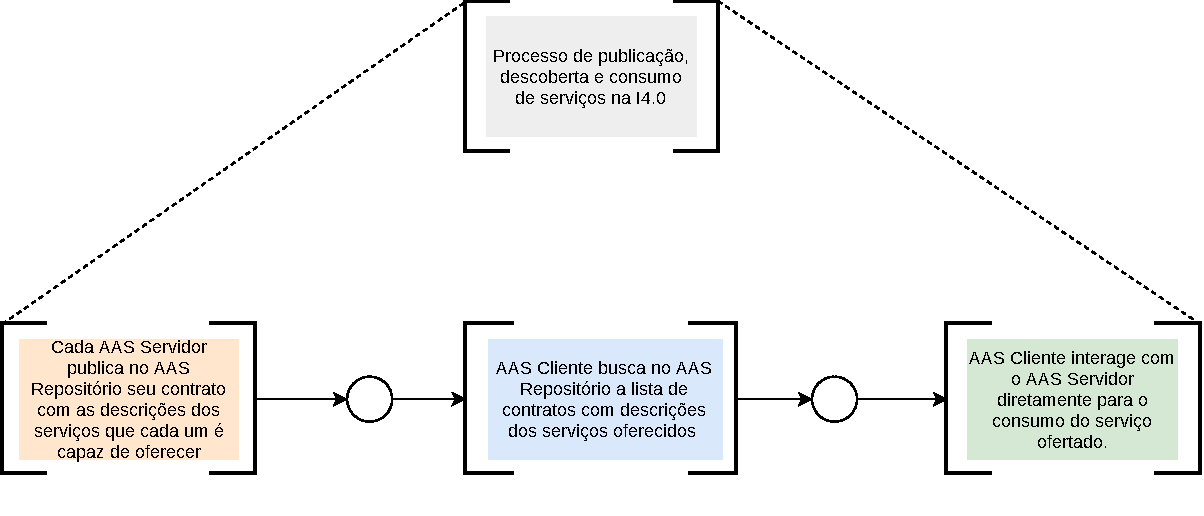
\includegraphics[width=1\textwidth]{pfs-ws}
		\fonte{O autor.}
	\end{figure}
	
	Os serviços fornecidos por um AAS são diversos. Entretanto, neste trabalho serão tratados com ênfase aqueles serviços que têm como objetivo o compartilhamento de informações sobre o ativo que possam agregar valor ao produto ao longo de sua cadeia de suprimentos. Ou seja, os serviços que extraem informações da MDP do AAS e as fornecem, mediante autenticação, às partes solicitantes ao longo da cadeia de suprimentos.

\section{Estrutura do AAS}

	Nesta proposta de arquitetura de WS, o conceito de Memória Digital do Produto (MDP) é inserido dentro da Indústria 4.0 com o objetivo de se agregar valor ao produto por meio da possibilidade de acesso a informações sobre o ativo entre parceiros ao longo da cadeia de valor.
	
	Nesta seção são apresentados os detalhes sobre uma possível estruturação do AAS para que seja compatível com a proposta de compartilhamento de informações por meio de WSs.
	
	\subsection{Integração da MDP ao AAS}
	
	A MDP precisa ser integrada ao AAS para que possa ter a estrutura necessária para que seus dados sejam disponibilizados ao mundo conectado da I4.0. A MDP em um AAS corresponde à organização dos dados do ativo, ao gerenciamento desses dados e às funções básicas aplicadas em cima desses dados. A MDP é uma \textit{view}, ou seja, ela replica e agrega as informações referentes a cada um dos submodelos de um AAS e as organiza de forma a poderem ser facilmente disponibilizadas por meio de WSs.
	
	Como a MDP é parte integral do AAS, que representa a parte virtual do ativo, esta pode ser fornecida em qualquer meio digital, inclusive em plataformas de serviços de computação em nuvem. Estas plataformas específicas suportam o armazenamento de grandes quantidades de dados, assim como podem assegurar uma alta capacidade de processamento de requisições de serviços.
	
	As informações contidas na MDP devem ser estruturadas de tal forma que simplifique a interpretação destes dados do lado do cliente. Para isso, metamodelos devem ser estabelecidos a fim de se criar moldes sobre os quais os dados devem ser estruturados.
	
	\citeonline{bader2019aas} estabelece padrões de metamodelos para a implementação de submodelos no AAS, porém não aborda um possível repositório de serviços e o armazenamento de descrições de serviços. A \autoref{tab:mdp-repositorio} traz uma proposta de metamodelo para a MDP do AAS Repositório para o armazenamento de descrições de serviços.
	
	\begin{table}[htb]
		\centering
		\caption{Proposta de metamodelo para a MDP do repositório.}
		\label{tab:mdp-repositorio}
		\begin{tabular}{p{3cm}p{12cm}}
			\hline
			\textbf{Propriedade}
			& \textbf{Descrição} \\ 
			
			\hline
			ID do AAS servidor
			& Tem a função de distinguir exclusivamente os AASs provedores de serviços e todos seus elementos \cite{adolphs2016structure} no mundo conectado da I4.0. Alguns tipos possíveis de identificadores são \cite{bader2019aas}: IRDI, IRI e UUID. O ID do AAS servidor é uma referência ao AAS Repositório e a todos os demais AASs que solicitarem a descrição dos serviços. \\
			
			\hline
			ID do serviço
			& Identificação exclusiva do serviço para a sua identificação única entre todos os repositórios. O ID do serviço pode ser derivado do próprio ID do AAS servidor com identificações extra do ID dentro do AAS (E.g., ID\_MODELO.SERVIÇO\_001). \\
			
			\hline
			Descrição do AAS provedor
			& Breve descrição sobre o AAS servidor e suas funções. \\
			
			\hline
			Protocolos de comunicação e padrões de API
			& Definição dos protocolos de comunicação suportados pelo fornecedor daquele serviço, como, por exemplo, HTTP, MQTT, etc; assim como as especificações do padrão para a comunicação via API como, por exemplo, REST, SOAP, GraphQL, etc.   \\
		
			\hline
			Formato de intercâmbio
			& Formato de arquivo de intercâmbio de informações. Ex.: json, xml, yaml, aasx, etc.  \\
			
			\hline
			\textit{Timestamp} da inserção do serviço no repositório
			& Data e hora de inserção do serviço ao repositório. \\
			
			\hline
			Indicação de disponibilidade
			& Chave booleana indicando se o AAS servidor atualmente suporta requisições. Esta propriedade pode estar desatualizada caso o AAS Servidor sofra uma falha de comunicação. Em outros casos, o AAS Servidor pode voluntariamente indicar ao repositório que temporariamente não processará solicitações de serviços. \\
			
			\hline
			Quality of Service (QoS)
			
			& A métrica de qualidade de serviço (QoT) fornece indicadores sobre a qualidade do serviço prestado por um determinado AAS. O tempo médio de resposta do serviço baseado no tempo de resposta observado por diversas requisições executadas e a disponibilidade do AAS quando solicitado são índices que contribuição do QoS. Um índice para serviços de qualidade mais subjetiva pode ser criado baseado em avaliações de AAS Clientes que já consumiram o serviço.\\
			
			\hline
			Descrição do serviço
			& Descrição sobre o funcionamento do serviço juntamente com o tipo de resposta esperado.  \\			
			\hline
		\end{tabular}
		\fonte{O autor.}
	\end{table}
	
	A \autoref{tab:mdp-repositorio} é uma lista não exaustiva das propriedades necessárias para o armazenamento de um serviço, ela apenas apresenta uma ideia sobre os tipos de chaves básicas necessárias para identificação e invocação de um serviço na rede.
	
	O AAS Cliente na operação de busca fará uma requisição ao repositório ou a uma lista de repositórios e receberá (de cada um dos repositórios) por meio de uma API a lista de serviços com uma estrutura de dados contendo os atributos chave-valor mencionados na \autoref{tab:mdp-repositorio}.
	
	Já o metamodelo da MDP do AAS servidor possuirá uma estrutura diferente, uma vez que deverá possuir as funções de agregação necessárias para a geração de alguns atributos. Uma proposta de metamodelo para a MDP do AAS servidor é apresentada na \autoref{tab:mdp-servidor}.
	
	\begin{table}[htb]
		\centering
		\caption{Proposta de metamodelo para a MDP do servidor.}
		\label{tab:mdp-servidor}
		\begin{tabular}{p{4cm}p{11cm}}
			\hline
			\textbf{Propriedade/Função}
			& \textbf{Descrição} \\ 
			
			\hline
			ID do serviço
			& Identificação exclusiva do serviço para a sua identificação única entre todos os repositórios. \\
			
			\hline
			Extração de dados dos submodelos
			& Função que retorna os dados solicitados pelo serviço. \\
			
			\hline
			Organização dos dados
			& Funções de estruturação dos dados ao formato solicitado pelo serviço, nesta fase pode haver também funções de limpeza dos dados brutos extraídos dos submodelos. \\
			
			\hline
			\textit{Quality of Service} (QoS)
			& Função para cálculo e armazenamento do índice de qualidade de serviço (QoS) com base em métricas sobre serviços já prestados e avaliações de AAS clientes que já consumiram o serviço. \\
			
			\hline
			Atualização da descrição do serviço no repositório
			& Função que envia ao repositório da empresa a descrição atualizada dos serviços. \\
			
			\hline
			Repositório
			& Referência ao repositório da empresa onde o ativo se encontra. \\			
			\hline
		\end{tabular}
		\fonte{O autor.}
	\end{table}
	
	A \autoref{tab:mdp-servidor}, assim como os metamodelos da MDP do Repositório (\autoref{tab:mdp-repositorio}), faz uma listagem não exaustiva de suas propriedades, sendo possível a inserção de novas funcionalidades adicionais na implementação do AAS. O metamodelo proposto na tabela se relaciona às funções da MDP em gerar a descrição dos serviços. Além desta atividade, a MDP possui as funções convencionais de armazenamento e gerenciamento dos dados dos submodelos.
	
	Com a MDP, o AAS servidor será, portanto, o único responsável pela geração e atualização de todos os metadados referentes aos serviços de seu AAS.

	
	\subsection{Detalhamento das partes do AAS}

	Nesta subseção é apresentada uma proposta de detalhamento dos elementos de um AAS contendo todas as partes necessárias para a implementação da arquitetura de compartilhamento de serviços baseada no RAMI4.0. 
	
	A estrutura proposta do AAS é baseda em \citeonline{bader2019aas}, que estabelece a divisão do AAS em submodelos e o divide em duas partes: o cabeçalho (\textit{header}) e o corpo (\textit{body}).
	
	O cabeçalho na estrutura proposta terá a função de providenciar informações públicas sobre o ativo que o identifiquem minimamente e que forneça uma descrição sobre seus serviços oferecidos. O cabeçalho deverá conter informações que podem ser acessadas sem a necessidade de autenticação, como, por exemplo, seu identificador único universal (UUID - \textit{Universal Unique IDentifier}), o modelo e fabricante do ativo. O cabeçalho deverá conter também a descrição dos serviços fornecidos por seus submodelos. A descrição dos serviços é enviada ao repositório ou pode ser também consultada diretamente pelo AAS solicitante.
	
	A descrição de cada serviço no cabeçalho deverá conter também referências ao próprio AAS como forma de referência para que, assim, o AAS Cliente possa localizar, contactar e invocar o serviço ofertado.
	
	O cabeçalho não terá a função de fornecer uma ficha técnica detalhada, mas apenas uma caracterização abstrata do ativo. O cabeçalho deverá necessariamente conter o UUID do AAS, sem o UUID o AAS se torna inacessível para qualquer uma das partes da cadeia de suprimentos.
	
	Dentro dos moldes da estrutura proposta, o corpo (\textit{body}) de um AAS fornece as informações e funcionalidades sensíveis sobre o ativo, que podem ser acessadas mediante autenticação. As funcionalidades dos ativos são agrupadas em forma de submodelos, conforme estabelecido em \citeonline{bader2019aas, adolph2018roadmap, bedenbender2017aasexamples}, que são unidades de agrupamento de funcionalidades semelhantes, como propriedades, serviços e demais regras de negócio do ativo. Os dados do ativo são armazenados nos próprios submodelos, enquanto a MDP (que também está contida no corpo do AAS) extrai e organiza as informações dos submodelos de forma a estruturá-las para serem diretamente fornecidas ao serviço.
	
	O corpo do AAS representa a carga útil (\textit{payload}) do AAS, pois é a porção de informação que é de fato relevante para o cliente que consumirá os serviços ofertados.
	
	A estrutura de um AAS compatível com a arquitetura orientada a serviços proposta é apresentada na \autoref{fig:estrutura-aas}.
	
	\begin{figure}[htb]
		\centering
		\caption{Estrutura do AAS com seus submodelos e a MDP.}
		\label{fig:estrutura-aas}
		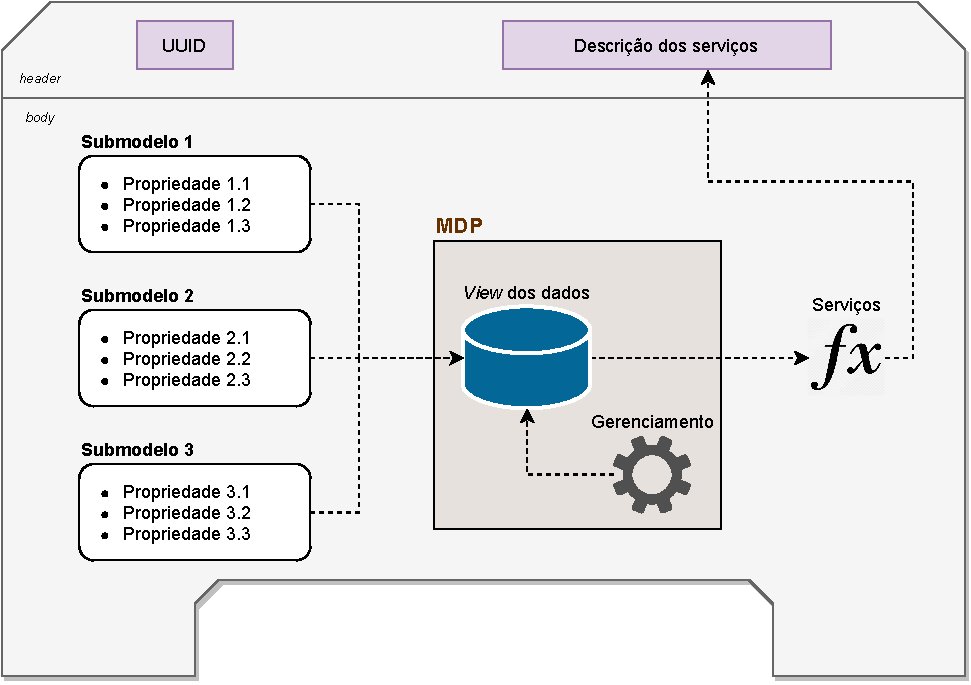
\includegraphics[width=0.7\textwidth]{estrutura-aas}
		\fonte{O autor.}
	\end{figure}

	Os dados contidos nos submodelos, quando processados pela MDP, fornecem informações úteis sobre o ativo e agregam valor ao mesmo. Além disso, novos modelos de negócio surgem sob os dados gerados pelo ativo.
	
	Neste trabalho é dado enfoque aos submodelos que se relacionam a informações sobre o produto que sejam de interesse a qualquer uma das partes ao longo da cadeia de suprimentos e que possam ser lidos ou escritos por meio dos WSs. Alguns exemplos desse tipo de submodelo podem incluir: a ficha técnica detalhada do ativo, submodelos de histórico de leitura de sensores, histórico de leitura de geolocalização (GPS), histórico de padrões de uso, etc.


\section{Fluxo de fornecimento de serviços}

	As etapas para o fornecimento de serviços na I4.0 segue um fluxo padrão. Os submodelos agregam informações semelhantes que podem ser lidas ou escritas por qualquer uma das partes ao longo da CS mediante autenticação.
	
	Um fluxo de leitura/escrita de dados pode ser exemplificado com uma CS simples contendo três membros: um fabricante, um distribuidor e um consumidor; cada membro da CS é AAS Cliente diferente. O fabricante cria o produto, que será o AAS Servidor, e define a estrutura de seu AAS e seus submodelos necessários, três submodelos são definidos: submodelo ``Geolocalização'', submodelo ``Sensores'' e submodelo ``Documentação''. Ao longo do ciclo de vida do produto, os membros da CS (fabricante, distribuidor e consumidor) podem interagir com esses submodelos, fazendo sua leitura para o caso dos submodelos de geolocalização e sensores, e podendo fazer a leitura e/ou escrita para o caso do submodelo de documentação.
	
	A \autoref{fig:webservice-multielo} demonstra este cenário mencionado com o fluxo de operações básicas do WS em funcionamento. Neste exemplo, o AAS de um produto \textbf{(a)} mantém contato com o AAS da empresa do fabricante \textbf{(b)}, com o AAS da empresa do distribuidor \textbf{(c)} e com o AAS do consumidor final \textbf{(d)}, fornecendo o serviço de consulta de informações de diferentes submodelos para cada um dos solicitantes. 	
	
	\begin{figure}[htb]
		\centering
		\caption{Exemplificação das operações de publicação e busca com múltiplos clientes.}
		\label{fig:webservice-multielo}
		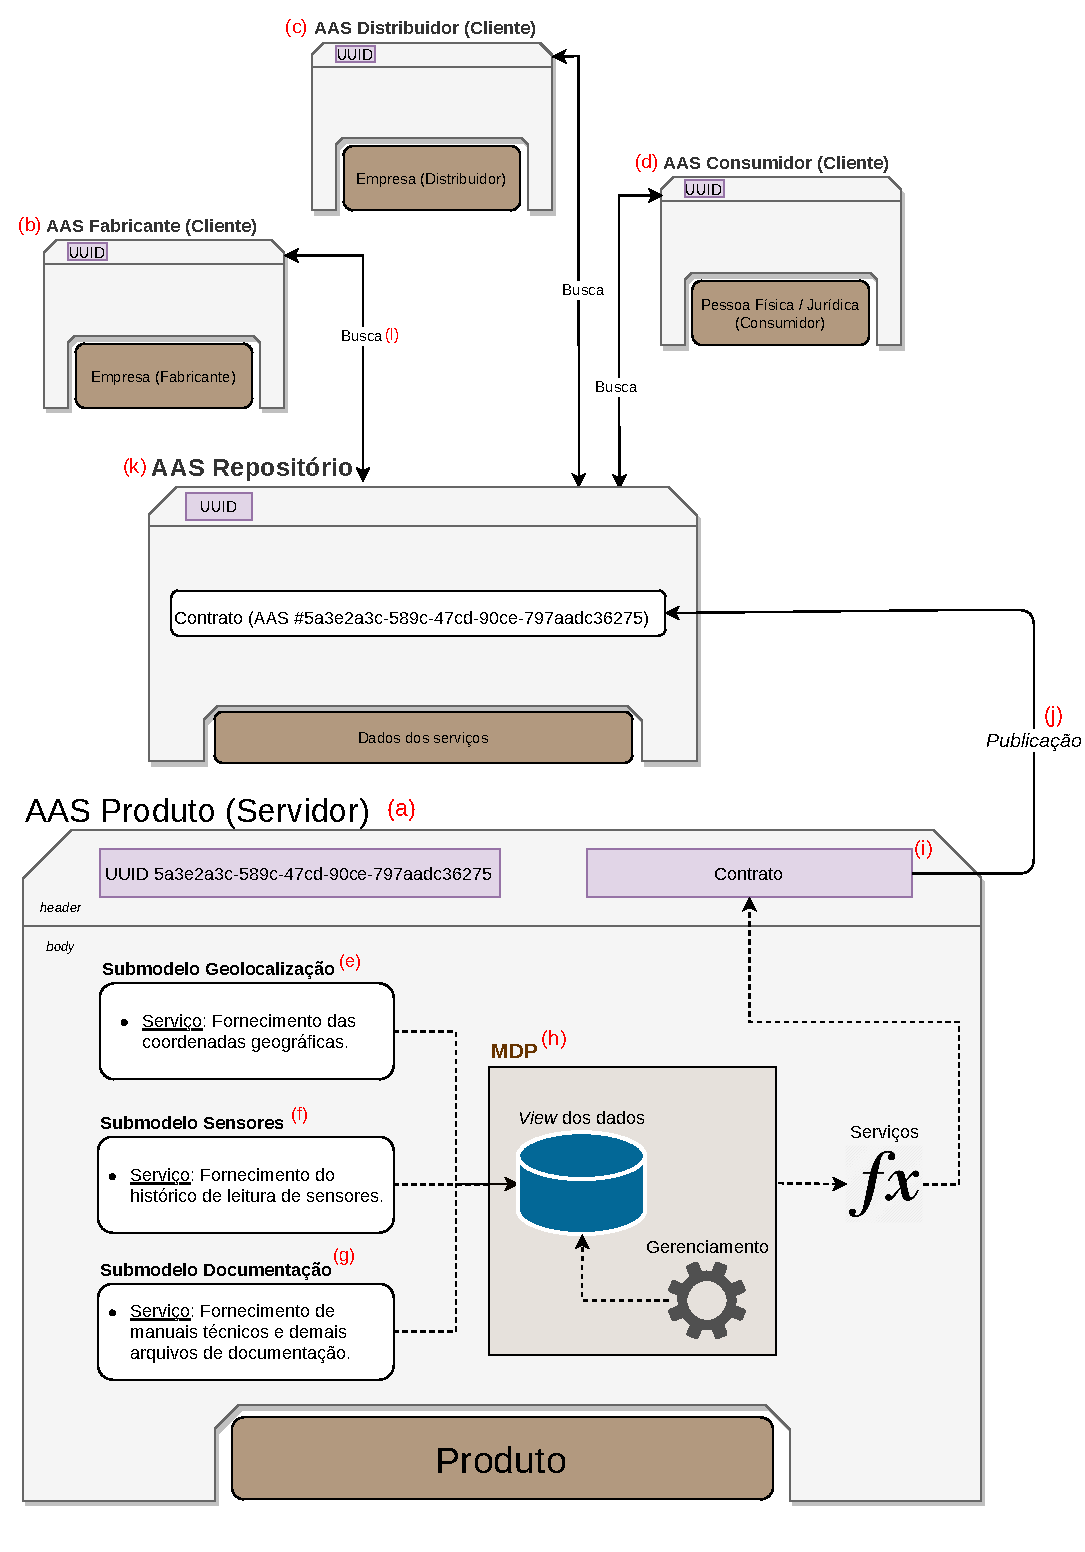
\includegraphics[width=0.8\textwidth]{webservice-multielo}
		\fonte{O autor.}
	\end{figure}

	Na \autoref{fig:webservice-multielo} são mostrados os três modelos dos AAS Produto: Submodelo ``geolocalização'' \textbf{(e)}, submodelo ``sensores'' \textbf{(f)} e submodelo ``documentação'' \textbf{(g)}. Os serviços de todos os submodelos disponíveis são mapeados pelas funções da MDP \textbf{(h)} e, assim, é gerada uma lista de descrições de serviços \textbf{(i)}. Esta lista de descrições de serviços é publicada \textbf{(j)} no repositório.
	
	O repositório \textbf{(k)} recebe a descrição de serviços do AAS Produto e as disponibiliza para consulta. O repositório receberá também listas de descrição de serviços de diversos outros AASs.
	
	Os AAS Clientes fazem a busca \textbf{(l)} no repositório. As buscas são feitas com parâmetros a fim de se restringir qual tipo de serviço aquele cliente pretende consumir, podendo-se restringir a busca, inclusive, ao serviço de um AAS específico, identificando-o por meio de seu UUID.
	
	Cada AAS Cliente (Fabricante, Distribuidor ou Consumidor), portanto, realiza a consulta ao AAS Repositório com os seus parâmetros de interesse e recebe a resposta com descrições detalhadas sobre os serviços disponíveis e informações para localizar, contactar e invocar estes serviços.
	
	O próximo passo após o recebimento da resposta do repositório é a decisão interna de cada AAS Cliente sobre qual serviço selecionar. Uma vez definido, o AAS Cliente estabelece uma comunicação direta com o AAS Servidor (produto) para o consumo do serviço selecionado.
	
	Este é um exemplo de consulta única. Em aplicações reais, o cliente normalmente invocaria o serviço de diversos AAS Servidores ao mesmo tempo, como, por exemplo, um fabricante solicitando informações de todas as máquinas de um modelo específico que foram vendidas a clientes espalhados pelo mundo para se realizar análise de dados a fim de se fazer uma manutenção preditiva por meio da identificação de potenciais falhas. Tal exemplo é demonstrado na \autoref{fig:webservice-multiproduto}.
	
	\begin{figure}[htb]
		\centering
		\caption{Exemplificação das operações de publicação e busca com múltiplos produtos.}
		\label{fig:webservice-multiproduto}
		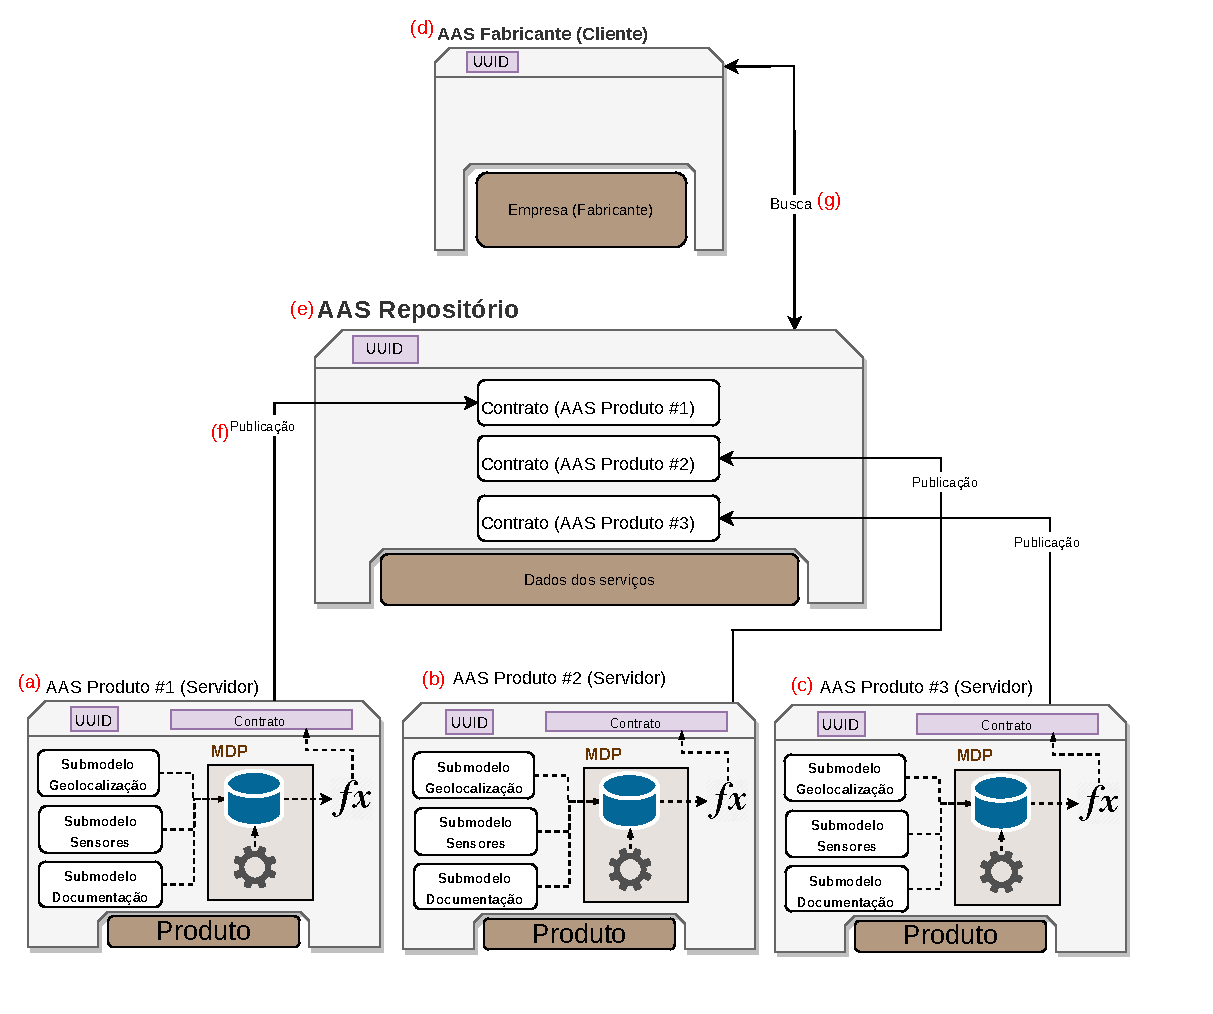
\includegraphics[width=1\textwidth]{webservice-multiproduto}
		\fonte{O autor.}
	\end{figure}

	
	A \autoref{fig:webservice-multiproduto} demonstra a situação de uma consulta de um AAS Cliente em múltiplos produtos. Neste exemplo, cada AAS Produto (\textbf{a}, \textbf{b} e \textbf{c}) realiza uma operação de publicação (\textbf{f}) no AAS Repositório (\textbf{e}). 
	
	O AAS Servidor (Fabricante) (\textbf{d}) por sua vez faz uma busca no AAS Repositório especificando os parâmetros que restrinjam a pesquisa a somente determinados modelos de produtos e recebe como resposta todas as descrições dos serviços que correspondem aos critérios de busca.	
	
	Todas as atividades de invocação de serviços na fase de interação são feitas mediante autenticação. É responsabilidade das funções da MDP realizar a autenticação ou bloqueio dos serviços disponíveis de acordo com as políticas de acesso de cada AAS.
	
	É importante notar que no mundo da I4.0 todo ativo é englobado por um AAS e se torna um Componente I4.0. Como o repositório detém informações e funções que agregam valor ao negócio, este pode também ser considerado um ativo e, portanto, possui o seu próprio AAS, que é responsável por toda a parte virtual deste ativo.
	
\section{Mapeamento das operações no RAMI4.0}
	
	Segundo \citeonline{iec2017rami}, o RAMI4.0 fornece uma visão estruturada dos principais elementos de um ativo usando um modelo de níveis composto por três eixos. Desta forma, inter-relações complexas podem ser divididas em seções menores e mais gerenciáveis, combinando os três eixos para representar cada aspecto relevante do estado do ativo em cada ponto de seu ciclo de vida.
	
	Esta seção tem o objetivo de mapear as operações do WS para dentro das camadas do RAMI4.0 de forma a representar todas as etapas do fluxo de informações em um modelo unificado.
	
	O mapeamento para o RAMI4.0, que é uma arquitetura de referência para a I4.0, contribui para facilitar a execução de implementações de conceitos de I4.0 uma vez que estabelece um padrão de arquitetura que deve ser adotado por todos, garantindo a interoperabilidades entre os sistemas.

\subsection{Descrição das camadas do RAMI4.0}

	Na \autoref{sub:rami4} foram apresentados os detalhes do RAMI4.0 e o detalhamento de cada nível do eixo Camadas com suas funções gerais. Nesta subseção é apresentada cada camada com enfoque para suas funções específicas para as operações em um WS.

	A camada mais inferior, \textbf{Ativo} é onde estará o elemento real do Componente I4.0 (C4.0) como, por exemplo, máquinas, sensores, pessoas, etc; e qualquer outro elemento, físico ou não, que represente valor ao negócio. O ativo será a fonte de dados, os quais serão compartilhados por meio de serviços para as partes ao longo da cadeia de suprimentos.
	
	Para o compartilhamento de informações do produto no mundo I4.0, os dados a serem extraídos do ativo são estrategicamente selecionados como o objetivo de reunir somente os dados que possam agregar valor ao próprio ativo. Assim, estes dados selecionados são extraídos do ativo e repassados às camadas superiores até que cheguem na camada Informação, onde são armazenados nos submodelos.
	
	Cada elemento desta camada, os ativos, deve possuir meios de comunicação e identificadores únicos (UUID), para permitir o seu monitoramento e supervisão dos dispositivos de controle por meio do AAS \cite{adolphs2015rami}.
	
	Na arquitetura orientada a serviços, três tipos de ativos básicos podem ser elencados: o produto, que é a fonte de dados e fornecedor dos serviços (servidor); as empresas ou pessoas, que são os clientes que consomem as informações da MDP do produto e também podem alterá-la; e as descrições dos serviços (WSD), que é o ativo encapsulado pelo C4.0-Repositório, responsável por garantir a visibilidade de um produto na cadeia de suprimentos.
	
	Na camada \textbf{Integração} estão as funcionalidades responsáveis pela virtualização de todos os ativos da camada inferior \cite{adolphs2015rami}. Ela representa a ponte para a troca de informações entre o mundo real e o virtual.
	
	Na arquitetura proposta para o compartilhamento de informações do ativo, esta camada está presente no CI4.0-Servidor, pois é dele que serão extraídos os dados desde o ativo até as camadas superiores. Tanto o C4.0-Cliente quanto o C4.0-Repositório operam primariamente nas camadas virtuais, porém também possuem a camada Integração, que faz a conexão com a empresa e o WSD, respectivamente. Esta camada adotará alguma tecnologias para a transferência de dados por meio físico como, por exemplo, o Wi-Fi, Ethernet, 5G, Bluetooth, etc.
	
	A camada \textbf{Comunicação} estabelecerá o protocolo de comunicação OPC UA para o C4.0-Servidor se comunicar com os demais C4.0s dentro da própria empresa (integração vertical).
	
	Para a arquitetura de compartilhamento de informações de ativos, não haverá comunicação entre C4.0s dentro da própria empresa uma vez que todas as operações de um WS (publicação, busca e interação) ocorrem entre componentes de organizações distintas. Ainda assim esta camada é necessária uma vez que ela define também os padrões de comunicação entre as camadas de um mesmo AAS.
	
	%É feito o pré-processamento de dados nesta fase, ou seja, antes de ser enviado para a camada Informação, onde será salvo nos submodelos. O pré-processamento dos dados inclui a remoção de redundâncias, duplicidades e remoção de \textit{outliers}.

	%Portanto, esta camada estabelece os protocolos de comunicação entre AASs dentro da mesma empresa (integração vertical), como os protocolos de comunicação entre AASs de diferentes empresas (integração horizontal). 

	A camada de \textbf{Informação} é onde os dados são de fato armazenados. Para isso, modelos de estrutura de Banco de Dados (BD) são definidos de acordo os tipos de dados e suas aplicações. Alguns exemplos de estrutura de dados incluem: BDs relacionais (e.g., MySQL, Postgres, SQLite) \cite{morris2017relationaldatabase} e demais BDs NoSQL como os orientados a documentos (e.g., MongoDB, CouchDB), os do tipo chave-valor (e.g., Redis, DynanoDB), os de armazenamento em coluna ampla (e.g., Cassandra, HBase) e os baseados em grafos (e.g.,Neo4j, JanusGraph) \cite{schaefer2019nosql}.
	
	Desta forma, esta camada é responsável por gerar e armazenar o WSD dos serviços oferecidos por cada C4.0-Servidor. Além disso, esta camada contém a parte da MDP que realiza a autenticação dos C4.0s solicitantes, ou seja, realiza o controle de acesso a suas informações.
	
	Na camada \textbf{Funcional} é onde ocorre toda a interação horizontal com C4.0s contidos no mundo conectado da I4.0. Esta camada é responsável pela integração horizontal entre as partes da cadeia de suprimentos de um produto. Os serviços são disponibilizados por meio da camada funcional, portanto é a interface entre os C4.0s de diferentes empresas.
	
	Esta camada deve definir o tipo de protocolo a ser utilizado para o fornecimento dos \textit{Web Services}, o protocolo HTTP é o mais comumente adotado para o fornecimento de WSs \cite{gruner2016restful}. Outros protocolos de aplicação também podem ser adotados como, por exemplo, o MQTT \cite{yokotani2016mqtt}.
	
	O fornecimento de serviços ao longo da cadeia de suprimentos é considerado uma integração horizontal uma vez que cada parte da CS representa uma organização diferente. Para o fornecimento e consumo desses serviços de compartilhamento de informações, devem ser definidas também as especificações da API, ou seja, o padrão de requisição e resposta para o fornecimento e consumo de serviços como, por exemplo, o padrão REST.
			
	A última camada, \textbf{Regra de Negócio}, é onde estão contidas as restrições legais e as políticas internas da empresa a serem aplicadas ao AAS \cite{adolphs2015rami}. No contexto da arquitetura de compartilhamento de informações do ativo baseada em \textit{Web Services}, esta camada conterá as restrições aplicadas sobre os serviços, como as políticas de privacidade de dados (E.g., restrições de acesso a determinados serviços) e as restrições legais de cada país.
	
	A regra de negócio estabelecerá quem na cadeia de suprimentos terá permissão para acessar quais informações do produto e quando. Um fabricante, por exemplo, terá acesso aos dados de padrões de uso de um produto somente sob a permissão do consumidor, o que representa uma regra nesta camada. Um distribuidor, por sua vez, só poderá ter acesso à localização do produto enquanto o produto estiver sob sua custódia.
	
	Outro ponto relevante desta camada para a arquitetura de compartilhamento de informações ao longo da CS são as condições legais de cada país, que criam restrições sobre o fornecimento de serviços, principalmente no aspecto de governança de dados.
	
	%Para os WSs, outra função importante desta camada é a orquestração dos serviços, que se refere ao gerenciamento dos serviços oferecidos. Quando os serviços são oferecidos em forma de contêineres, o orquestrador de serviços permite a escalabilidade da capacidade de trabalho, permitindo a invocação ou remoção de contêineres de acordo com a demanda de um determinado serviço. Alguns orquestradores de contêineres podem ser citados, como o Kubernetes, Docker Swarm e Apache Mesos \cite{redhat2020orchestration}.
	
	O conjunto de todas estas camadas representa um \textbf{Componente I4.0} (C4.0). Para cada tipo de operação relacionada a um componente, é necessário detalhar o fluxo de dados e de eventos acontecendo em cada uma das camadas. Este detalhamento permite que implementações de soluções I4.0 sejam facilitadas e garante que a criação dessas soluções por diversos desenvolvedores de sistemas resulte em sistemas que sejam interoperáveis, independentemente da tecnologia adotada.
	
	O \textbf{Componente I4.0} pode ainda ser mais detalhadamente especificado, identificando se o componente representa um produto em desenvolvimento ou uma instância de um produto já fabricado. Estes detalhes são cobertos pelo eixo Ciclo de Vida e Cadeia de Valor e considerações sobre este eixo envolvendo a arquitetura proposta baseada em WSs é apresentada no \autoref{cha:ciclo-de-vida}.
	
	A \autoref{fig:webservice-rami} apresenta os componentes da arquitetura de fornecimento de WSs dentro do eixo Camadas do RAMI4.0, que são:
	
	\begin{itemize}
		\item \textbf{Ativo}: Pessoas e empresas (cliente), produtos (servidor) e WSDs (repositório); 
		\item \textbf{Integração}: Virtualização das informações, protocolos de transferência de dados (Ethernet, 5G, Wi-Fi, etc); 
		\item \textbf{Comunicação}: Protocolos de comunicação vertical (OPC UA); 
		\item \textbf{Informação}: Controle de acesso / autenticação, análise de dados, armazenamento, descrição dos serviços (virtual);
		\item \textbf{Funcional}: Serviços de compartilhamento de informações, protocolos de comunicação horizontal (HTTPS, MQTT, etc), interface horizontal entre AASs; 
		\item \textbf{Regra de negócio}: Restrições legais, políticas de privacidade.
	\end{itemize}
	
	\begin{figure}[H]
		\centering
		\caption{Camadas do RAMI4.0 com os elementos da arquitetura.}
		\label{fig:webservice-rami}
		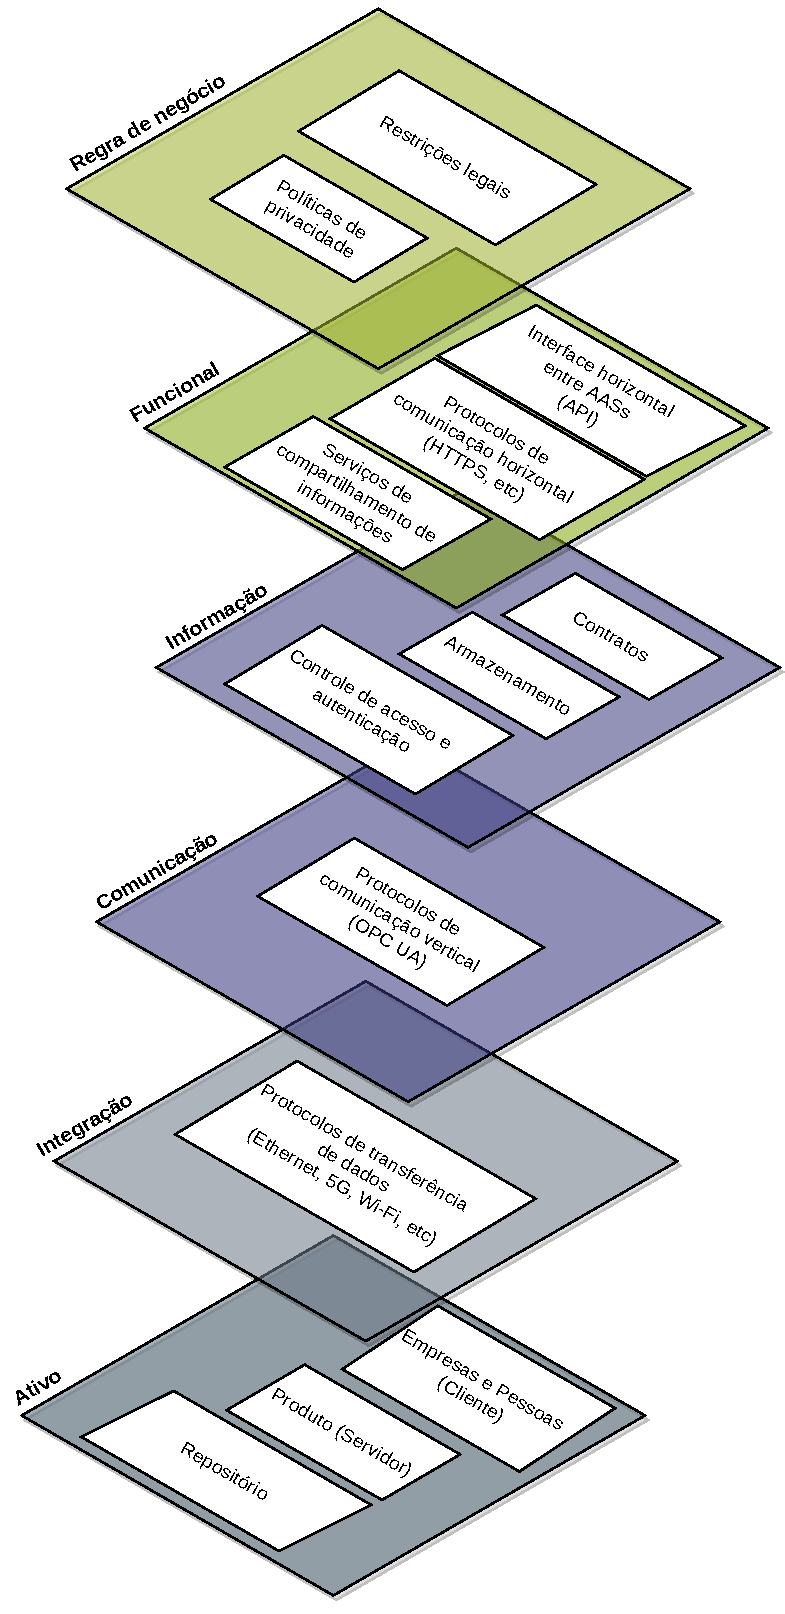
\includegraphics[width=0.7\textwidth]{webservice-rami}
		\fonte{O autor.}
	\end{figure}

\subsection{Operação de Publicação}

	A \autoref{fig:rami-publicacao} apresenta diagramas PFS do fluxo de atividades para a operação de publicação de um C4.0-Servidor em um C4.0-Repositório.
	
	\begin{figure}[htb]
		\centering
		\caption{Diagrama PFS da operação de publicação.}
		\label{fig:rami-publicacao}
		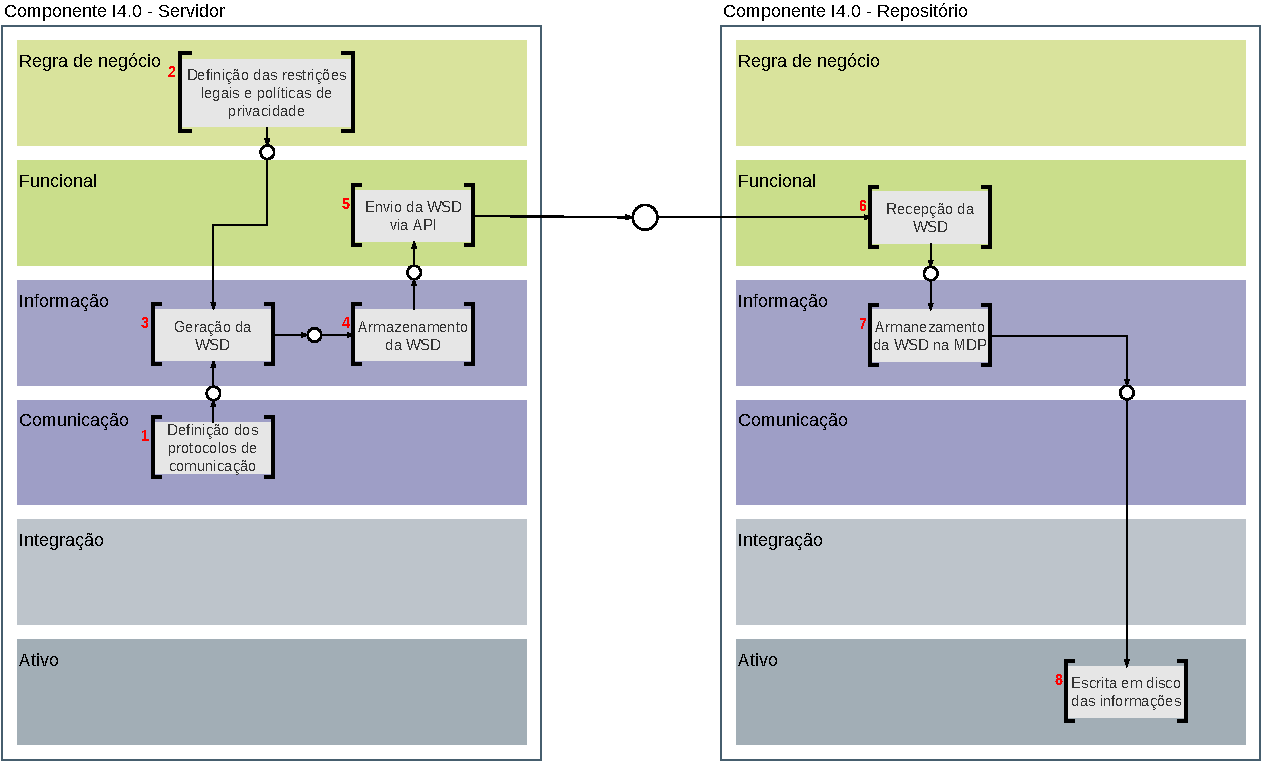
\includegraphics[width=1\textwidth]{rami-publicacao}
		\fonte{O autor.}
	\end{figure}

	Esta operação é iniciada pelo C4.0-Servidor, seguindo um fluxo de atividades estabelecido até chegar no ativo do C4.0-Repositório, os passos são detalhados a seguir:
	
	\begin{enumerate}
		
		\item As restrições legais e as políticas de privacidade para um determinado C4.0 são definidas e acessadas. Esta atividade adicionará restrições ao serviço a ser publicado. Estas restrições serão incorporadas à descrição de cada serviço a ser publicado.
		
		\item A geração da lista de descrições de serviços (WSD) é feita com base nos serviços disponíveis no C4.0-Servidor e nas restrições impostas na atividade anterior. Uma descrição de cada serviço ativo é gerada em um formato de intercâmbio padronizado.
		
		\item A MDP local componente armazena a lista de WSD nos submodelos.
		
		\item São definidos os protocolos de comunicação a serem utilizados na integração horizontal, assim como a especificação do padrão de requisição e resposta da API e o formato de intercâmbio de informações.
		
		\item A lista de WSD é enviada ao CI4.0-Repositório via API.
		
		\item O C4.0-Repositório recebe a lista de WSD no formato de intercâmbio definido. A descrição dos serviços nesta fase já contém todas as informações para a identificação do serviço e de seu componente correspondente.
		
		\item A lista de WSD é armazenada junto às demais descrições de serviços na MDP do C4.0-Repositório.
		
		\item São definidos os protocolos de comunicação vertical para a comunicação com as camadas inferiores.
		
		\item Os dados alimentam uma interface para comunicação com o ativo real.
		
		\item Os dados são escritos em disco.
	\end{enumerate}

\subsection{Operação de Busca}

	A operação de busca é dividida em duas partes: a requisição e a resposta. A requisição é a iniciativa do C4.0-Cliente para requerer a lista de WSD de um C4.0-Repositório. O fluxo de atividades da requisição em uma operação de busca é apresentado na \autoref{fig:rami-busca-requisicao}.
	
	Já a resposta da requisição em uma operação de busca é feita do C4.0-Repositório para o C4.0-Cliente e é apresentada na \autoref{fig:rami-busca-resposta}.
	
	\begin{figure}[htb]
		\centering
		\caption{Diagrama PFS da requisição em uma operação de busca.}
		\label{fig:rami-busca-requisicao}
		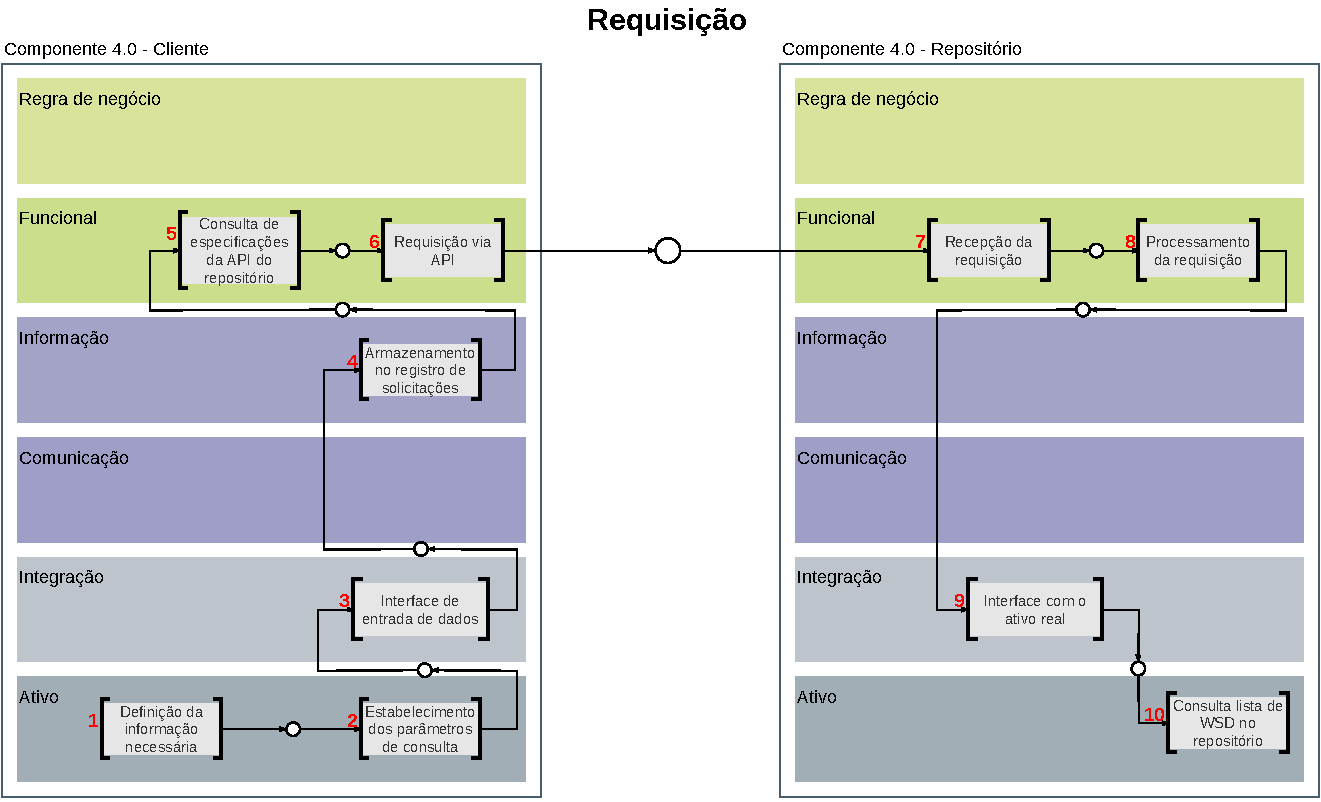
\includegraphics[width=1\textwidth]{rami-busca-requisicao}
		\fonte{O autor.}
	\end{figure}

	A operação de requisição para a busca de um serviço parte do C4.0-Cliente e segue um fluxo estabelecido até chegar ao C4.0-Repositório, esses passos são detalhados a seguir:
	
	\begin{enumerate}
		
		\item O processo de requisição começa com a definição por parte do ativo do C4.0-Cliente (pessoa ou empresa) da informação que se deseja consultar como, por exemplo, leituras de sensores, localização geográfica, manuais, etc. Essa definição pode ser manual, partindo da solicitação explícita de alguém, ou programática.
		
		\item A partir do tipo de informação a ser consultada, define-se os parâmetros de consulta, que representam o conjunto de restrições que estabelecem qual é exatamente o tipo de serviço que o AAS Cliente deseja consumir. Para os serviços que visam a extração de informações do ativo, os parâmetros representam, por exemplo, o ID do provedor de serviços, o horário e data de um determinado evento, uma filtragem por modelos específicos de um produto, etc.
		
		\item Os parâmetros de consulta alimentam uma interface para que a solicitação possa ser virtualizada e integrada ao AAS. Nesta atividade a intenção de solicitação de um serviço é virtualizada.
		
		\item São definidos os protocolos de comunicação vertical para a comunicação com as camadas superiores.
		
		\item A MDP local armazena os detalhes da solicitação em um registro de solicitações realizadas.
		
		\item São definidos os protocolos de comunicação a serem utilizados na integração horizontal, assim como a especificação do padrão de requisição e resposta da API e o formato de intercâmbio de informações.
		
		\item A requisição é enviada ao C4.0-Repositório via API.
		
		\item O C4.0-Repositório recebe a solicitação e a insere ao final da lista de solicitações para ser processada.
		
		\item A requisição é processada. Identifica-se nesta atividade se a requisição é válida e se ela contém todos os parâmetros necessários para a consulta.
		
		\item A MDP realiza a consulta à lista de WSDs utilizando os parâmetros de consulta estabelecidos.
		
		\item São definidos os protocolos de comunicação vertical para a comunicação com as camadas inferiores.
		
		\item Estabelece-se uma interface para a interação entre o AAS e seu ativo real.
		
		\item As informações solicitadas são lidas do disco e se tornam disponíveis para envio.
	\end{enumerate}

	Após a requisição, o C4.0-Repositório envia a resposta ao C4.0-Cliente. O fluxo de atividades da resposta é apresentada em diagramas PFS na \autoref{fig:rami-busca-resposta}.

	\begin{figure}[htb]
		\centering
		\caption{Diagrama PFS da resposta em uma operação de busca.}
		\label{fig:rami-busca-resposta}
		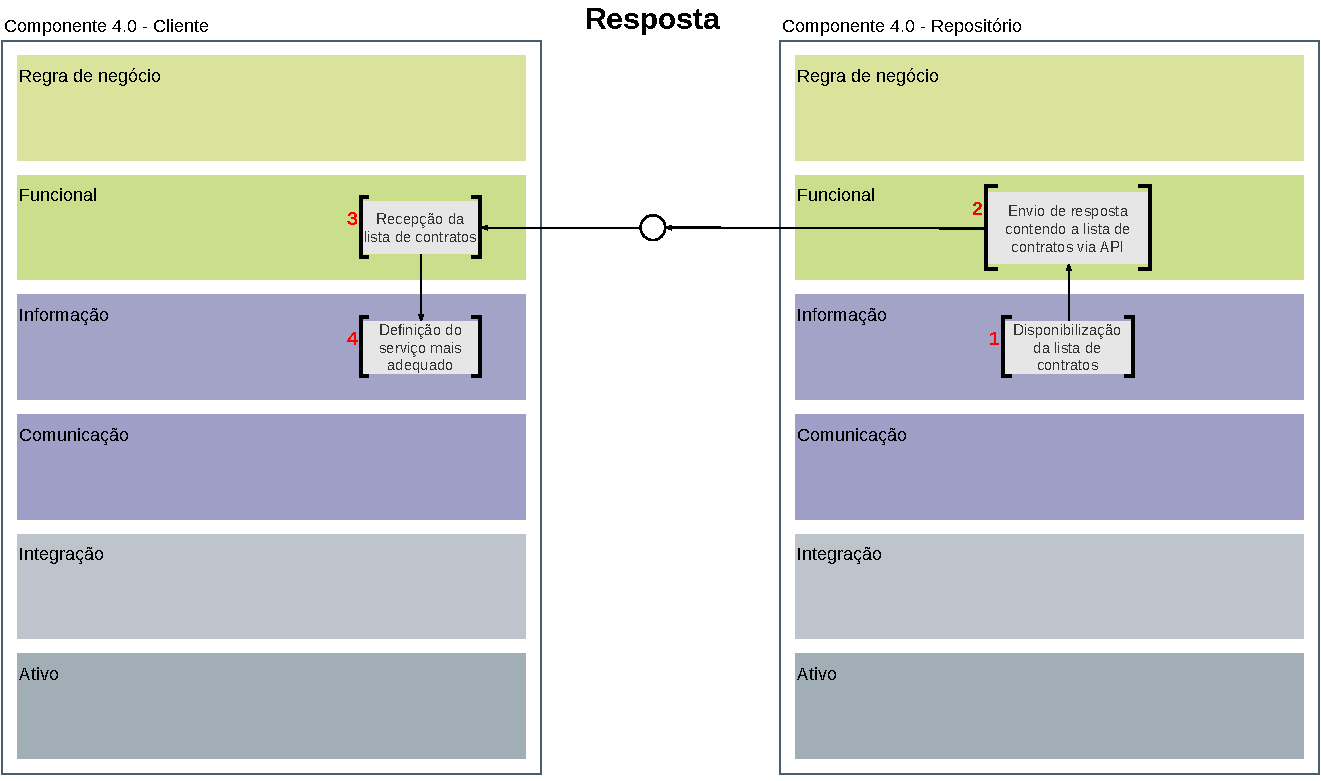
\includegraphics[width=1\textwidth]{rami-busca-resposta}
		\fonte{O autor.}
	\end{figure}

	Detalhadamente, a resposta do AAS Repositório segue o seguinte fluxo de atividades, começando pela disponibilização das informações reais do ativo repositório:
	
	\begin{enumerate}
		\item Os dados do ativo (WSD) são disponibilizados para consulta pelas camadas superiores.
		
		\item Os dados disponibilizados são virtualizados para a integração com o AAS.
		
		\item São definidos os protocolos de comunicação vertical para a comunicação com as camadas superiores.
		
		\item É realizada a consulta da lista de WSDs. Os resultados podem ser uma lista de serviços válidos, assim como podem conter mensagens de erro devido a solicitações inválidas ou buscas retornando zero correspondências.
		
		\item A lista de WSD é disponibilizada para acesso por parte da camada Funcional.
		
		\item São definidos os protocolos de comunicação a serem utilizados na integração horizontal, assim como a especificação do padrão de requisição e resposta da API e o formato de intercâmbio de informações.

		\item A resposta é enviada ao C4.0-Cliente via API.
		
		\item O C4.0-Cliente recebe a resposta contendo a lista de WSD em um formato de intercâmbio definido.
		
		\item Após a recepção da lista de serviços disponíveis, é feito o processamento para a definição do serviço mais adequado. Em consultas a serviços de compartilhamento de informações esta fase é simplificada, uma vez que os próprios parâmetros de consulta na requisição já definem o serviço ideal que o cliente busca. A seleção do serviço mais adequado é baseada nos parâmetros definidos na operação de requisição, que estabelecem os requisitos do serviço.
	\end{enumerate}

\subsection{Operação de Interação}

	A operação de interação é a fase final para o consumo de um serviço disponibilizado no mundo conectado da I4.0. Assim como a busca, a interação é divida em requisição e resposta. Primeiramente, o C4.0-Cliente faz uma requisição de consumo de um serviço com parâmetros e então a requisição é processada e respondida pelo C4.0-Servidor.
	
	 A \autoref{fig:rami-interacao-requisicao} apresenta o fluxo de atividades em uma requisição de um serviço e a \autoref{fig:rami-interacao-resposta} a resposta do serviço.
	
	\begin{figure}[htb]
		\centering
		\caption{Diagrama PFS da requisição de um serviço em uma operação de interação.}
		\label{fig:rami-interacao-requisicao}
		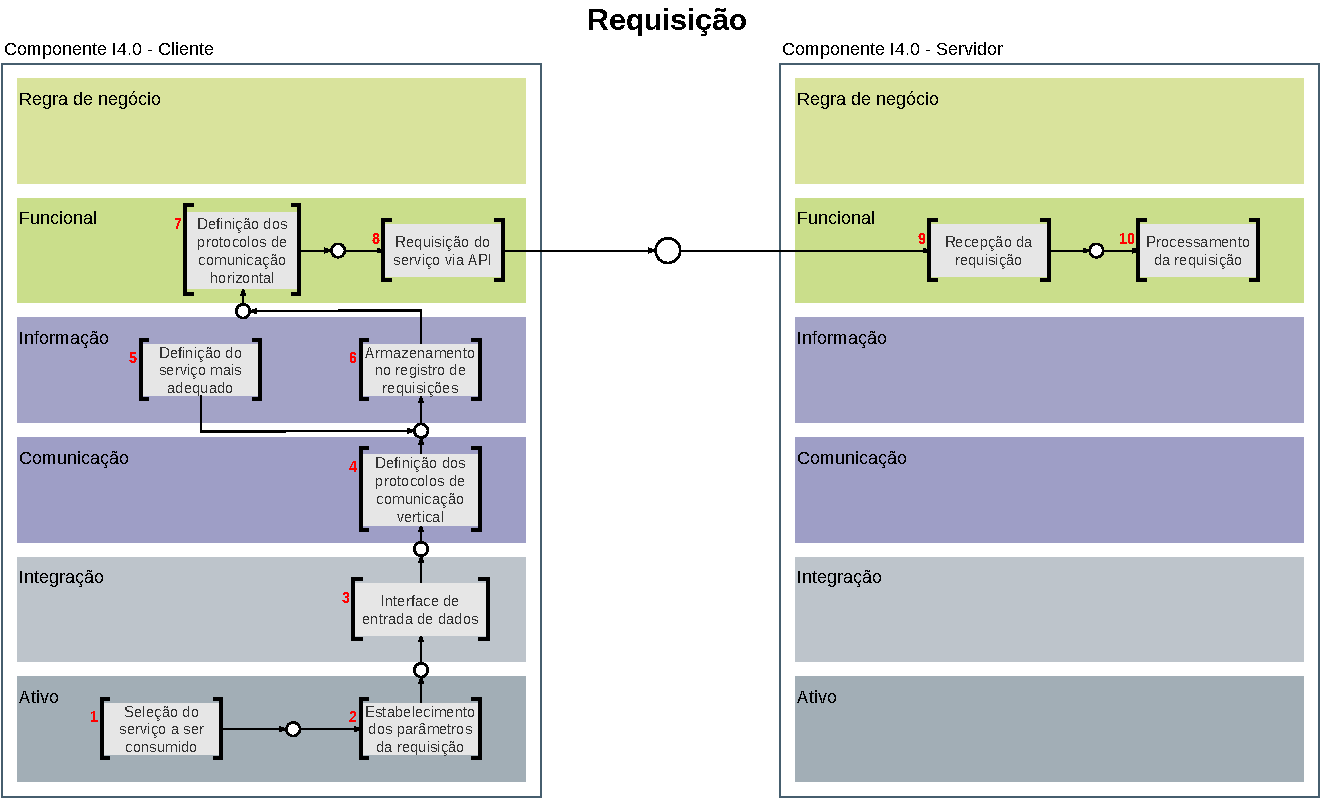
\includegraphics[width=1\textwidth]{rami-interacao-requisicao}
		\fonte{O autor.}
	\end{figure}

	A requisição de um serviço na operação de interação é iniciada pelo C4.0-Cliente e é enviada diretamente ao C4.0-Servidor usando a WSD fornecida pelo C4.0-Repositório. O fluxo de atividades para a requisição de um serviço é detalhada a seguir:
	
	\begin{enumerate}
		
		\item O processo de requisição começa com a definição exata sobre qual serviço de qual C4.0 será consumido. Caso a decisão seja feita manualmente, a intenção de requisição começa pelo ativo do C4.0-Cliente (pessoa ou empresa) com a seleção do serviço.
		
		\item Define-se os parâmetros da requisição de um serviço, que representam as opções obrigatórias ou opcionais para o detalhamento do serviço a ser consumido.
		
		\item Os parâmetros de consulta alimentam uma interface para que a requisição possa ser virtualizada e integrada ao AAS. Nesta atividade a intenção de interação é virtualizada.
		
		\item São definidos os protocolos de comunicação vertical para a comunicação com as camadas superiores.
		
		\item O processo de requisição pode iniciar diretamente da camada Informação por meio de uma decisão autônoma sobre o serviço mais adequado, sem a necessidade de uma tomada de decisão manual por parte de uma pessoa/empresa.
		
		\item A MDP local armazena os detalhes da requisição em um registro de requisições realizadas.
		
		\item São definidos os protocolos de comunicação a serem utilizados na integração horizontal, assim como a especificação do padrão de requisição e resposta da API e o formato de intercâmbio de informações.
		
		\item A requisição do serviço é enviada ao C4.0-Servidor via API.
		
		\item O C4.0-Servidor recebe a requisição e a insere ao final da lista de requisições para ser processada.
		
		\item A requisição é processada. Identifica-se nesta atividade se a requisição é válida e se ela contém todos os parâmetros necessários para o fornecimento do serviço.
		
	
	\end{enumerate}

	\begin{figure}[htb]
		\centering
		\caption{Diagrama PFS da resposta de um serviço em uma operação de interação.}
		\label{fig:rami-interacao-resposta}
		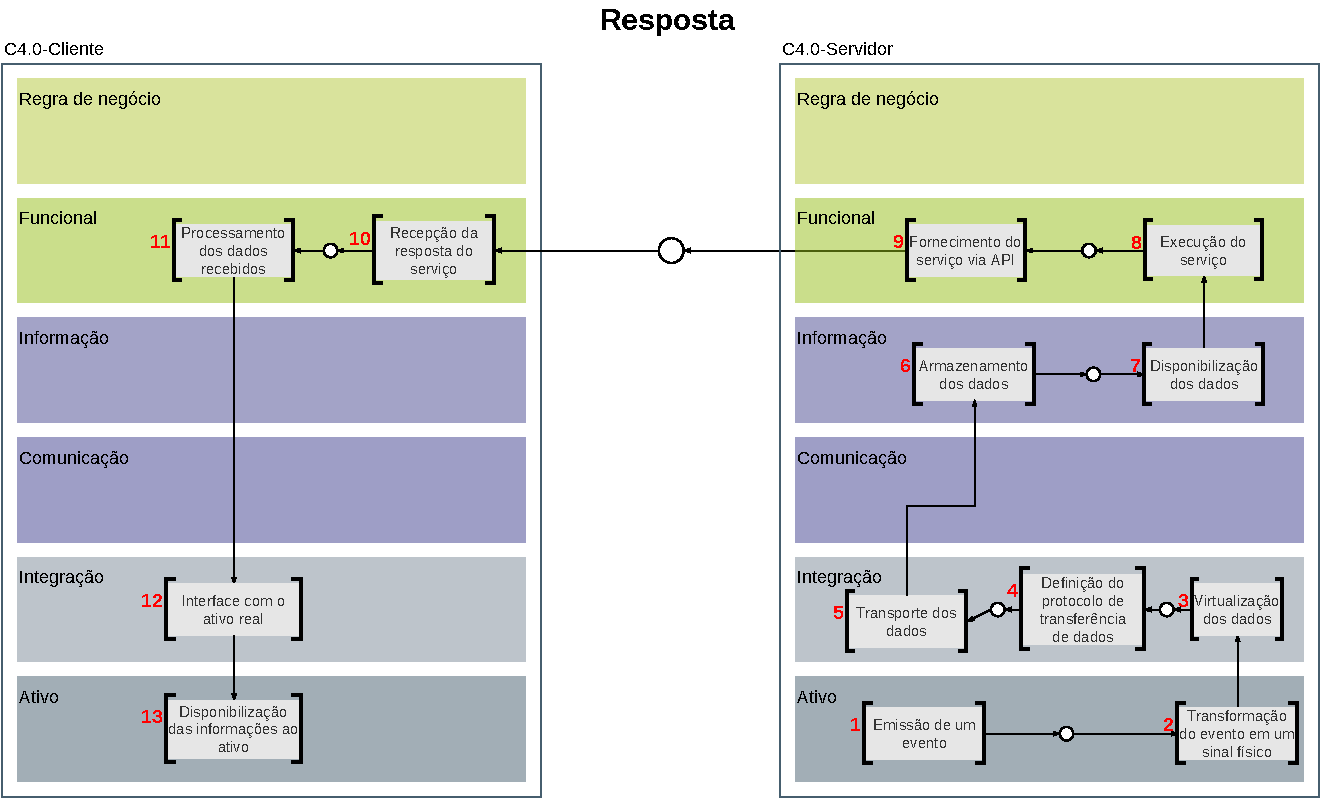
\includegraphics[width=1\textwidth]{rami-interacao-resposta}
		\fonte{O autor.}
	\end{figure}
	
	Após o recebimento e processamento da requisição de um serviço, o C4.0-Servidor deve fazer a extração e envio das informações do ativo. A resposta contendo as informações sobre o produto começa com a emissão de um evento no ativo. Esta informação percorre um fluxo padrão para que seja disponibilizada ao C4.0-Cliente por meio do serviço. Este fluxo de atividades mostrado na \autoref{fig:rami-interacao-resposta} é detalhado a seguir:
	
	\begin{enumerate}
		
		\item Um evento físico no mundo real é emitido.
		
		\item O evento fornece sinais físicos que podem ser medidos.
		 
		\item Os sinais físicos são interpretados e virtualizados. Nesta atividade é criado um correspondente virtual para o evento do ativo físico, ou seja, os dados são digitalizados e disponibilizados ao AAS.
		
		\item É definido o meio de transporte e o procolo de transferência de dados como, por exemplo, o Wi-Fi, Ethernet, 5G, etc.
		
		\item Os dados são devidamente transportados pelo meio e protocolo definidos até uma central de processamento.
		
		\item São definidos os protocolos de comunicação vertical para a comunicação com as camadas superiores.
		
		\item Os novos dados sobre o ativo são armazenados pela MDP nos submodelos junto aos demais dados já existentes.
		
		\item São definidas/acessadas as restrições legais e as políticas de privacidade para a autorização ou bloqueio do fornecimento do serviço.
		
		\item É feita a autenticação do C4.0-Cliente solicitante do serviço. Nesta atividade é verificado se o cliente possui autorização para consumir o serviço e consequentemente os dados que estão sendo solicitados.
		
		\item Após a autenticação, os dados são disponibilizados ao serviço.
		
		\item O serviço é executado e sua resposta é gerada. O serviço pode executar quaisquer operações sobre os dados atualizados sobre o ativo assim como sobre o histórico de registros antigos já disponíveis nos submodelos.
		
		\item São definidos os protocolos de comunicação a serem utilizados na integração horizontal, assim como a especificação do padrão de requisição e resposta da API e o formato de intercâmbio de informações.
		
		\item A resposta do serviço (fornecimento do serviço) é enviada via API.
		
		\item O C4.0-Cliente recebe a resposta do serviço no formato de intercâmbio definido.
		
		\item Os dados recebidos na resposta são processados.
		
		\item Opcionalmente a resposta e/ou resultados de processamento da resposta podem ser salvos na MDP local ou descartados.
	\end{enumerate}
	